\section{Assignment 3}

\subsection{Compute the canonical orientation of the 3D model}

The orientation of the point clouds and meshes produced by Zephyr is arbitrary. Since some 3D registration algorithms (e.g. ICP) require a strong initialization, a canonical orientation is introduced. The canonical orientation is derived from the covariance matrix of the point cloud, from which three principal directions are extracted using Principal Component Analysis (PCA).

\begin{figure}[h]
\centering
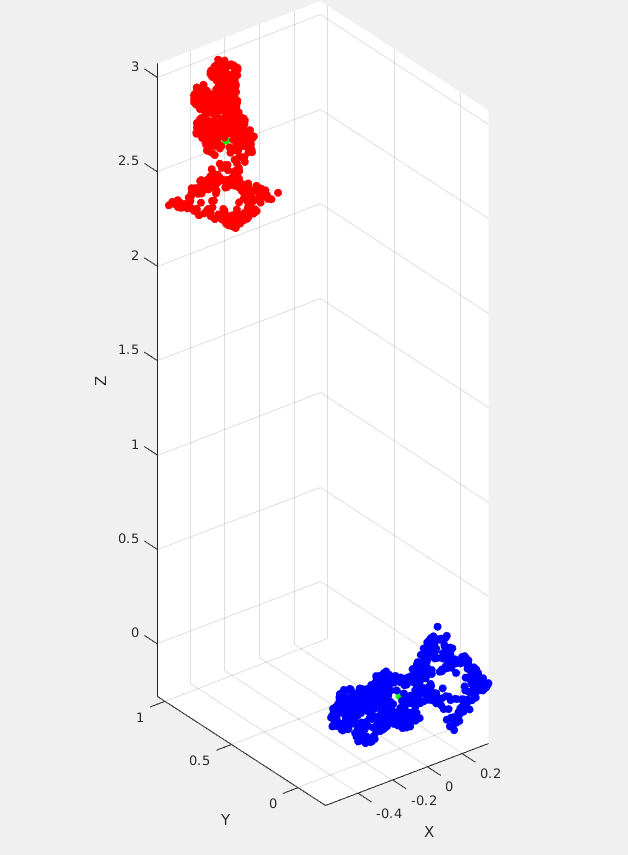
\includegraphics[keepaspectratio,width=0.7\textwidth]{canonical}
\caption{Zephyr orientation (red) vs canonical orientation (blue), centroids (green)}
\end{figure}